%----------------------------------------------------------------------------------------
%	PACKAGES AND OTHER DOCUMENT CONFIGURATIONS
%----------------------------------------------------------------------------------------

\documentclass[11pt]{diazessay} % Font size (can be 10pt, 11pt or 12pt)
\usepackage{float}
\usepackage{sectsty}
\usepackage{appendix}
\usepackage[numbers]{natbib}
\sectionfont{\centering}
\usepackage{listings}
\usepackage{color}

\definecolor{dkgreen}{rgb}{0,0.6,0}
\definecolor{gray}{rgb}{0.5,0.5,0.5}
\definecolor{mauve}{rgb}{0.58,0,0.82}

%\lstset{ 
%         language=Matlab,                                % choose the language of the code
%       basicstyle=10pt,                                % the size of the fonts that are used for the code
%         numbers=left,                                   % where to put the line-numbers
%         numberstyle=\footnotesize,                      % the size of the fonts that are used for the line-numbers
%         stepnumber=1,                                           % the step between two line-numbers. If it's 1 each line will be numbered
%         numbersep=5pt,                                  % how far the line-numbers are from the code
%       backgroundcolor=\color{white},          % choose the background color. You must add \usepackage{color}
%         showspaces=false,                               % show spaces adding particular underscores
%         showstringspaces=false,                         % underline spaces within strings
%         showtabs=false,                                         % show tabs within strings adding particular underscores
%       frame=single,                                           % adds a frame around the code
%       tabsize=2,                                              % sets default tabsize to 2 spaces
%       captionpos=b,                                           % sets the caption-position to bottom
%         breakatwhitespace=false,                        % sets if automatic breaks should only happen at whitespace
%         escapeinside={\%*}{*)}                          % if you want to add a comment within your code
%}

\lstset{frame=tb,
  breaklines=true,                                        % sets automatic line breaking
  language=php,
  aboveskip=3mm,
  belowskip=3mm,
  showstringspaces=false,
  columns=flexible,
  basicstyle={\small\ttfamily},
  numbers=none,
  numberstyle=\tiny\color{gray},
  keywordstyle=\color{blue},
  commentstyle=\color{dkgreen},
  stringstyle=\color{mauve},
  breaklines=true,
  breakatwhitespace=true,
  tabsize=3
}
%----------------------------------------------------------------------------------------
%	TITLE SECTION
%----------------------------------------------------------------------------------------

\title{\textbf{Traffic Analysis} \\ {\Large\itshape A write-up}} % Title and subtitle

\author{\textbf{Matthew Doherty \& Daniel de la Harpe} \\ \textit{Rhodes University}} % Author and institution

\date{\today} % Date, use \date{} for no date

%----------------------------------------------------------------------------------------

\begin{document}

\maketitle % Print the title section

%----------------------------------------------------------------------------------------
%	ABSTRACT AND KEYWORDS
%----------------------------------------------------------------------------------------

%\renewcommand{\abstractname}{Summary} % Uncomment to change the name of the abstract to something else

\renewcommand{\thesection}{\arabic{section}}
\renewcommand{\thesubsection}{\arabic{subsection}}
\renewcommand{\thesubsubsection}{\arabic{subsubsection}}
\renewcommand{\thesubsection}{\thesection.\arabic{subsection}}
\renewcommand{\thesubsubsection}{\thesubsection.\arabic{subsubsection}}

\vspace{30pt} % Vertical whitespace between the abstract and first section

%----------------------------------------------------------------------------------------
%	ESSAY BODY
%----------------------------------------------------------------------------------------

% "*" means no numbering -> \section*{Introduction}

\section*{Introduction}
This analysis examines events that took place on a South African network on the 2017-03-20 and 2017-03-22. We will make the argument, based purely on captured network traffic, that a host was compromised with a ransomware variant known as Maktub. Ransomware is the term used to describe malicious software that either encrypts data (thus denying access), or threatens to leak data. The attacker will offer to stop the attack if payment is received thus the name ransomware. Maktub is of the encryption variant and is usually delivered via an email attachment, which appears legitimate but performs its malicious activity in the background.



%------------------------------------------------

\section*{Traffic Overview}

\begin{figure}[H]
        \centering
        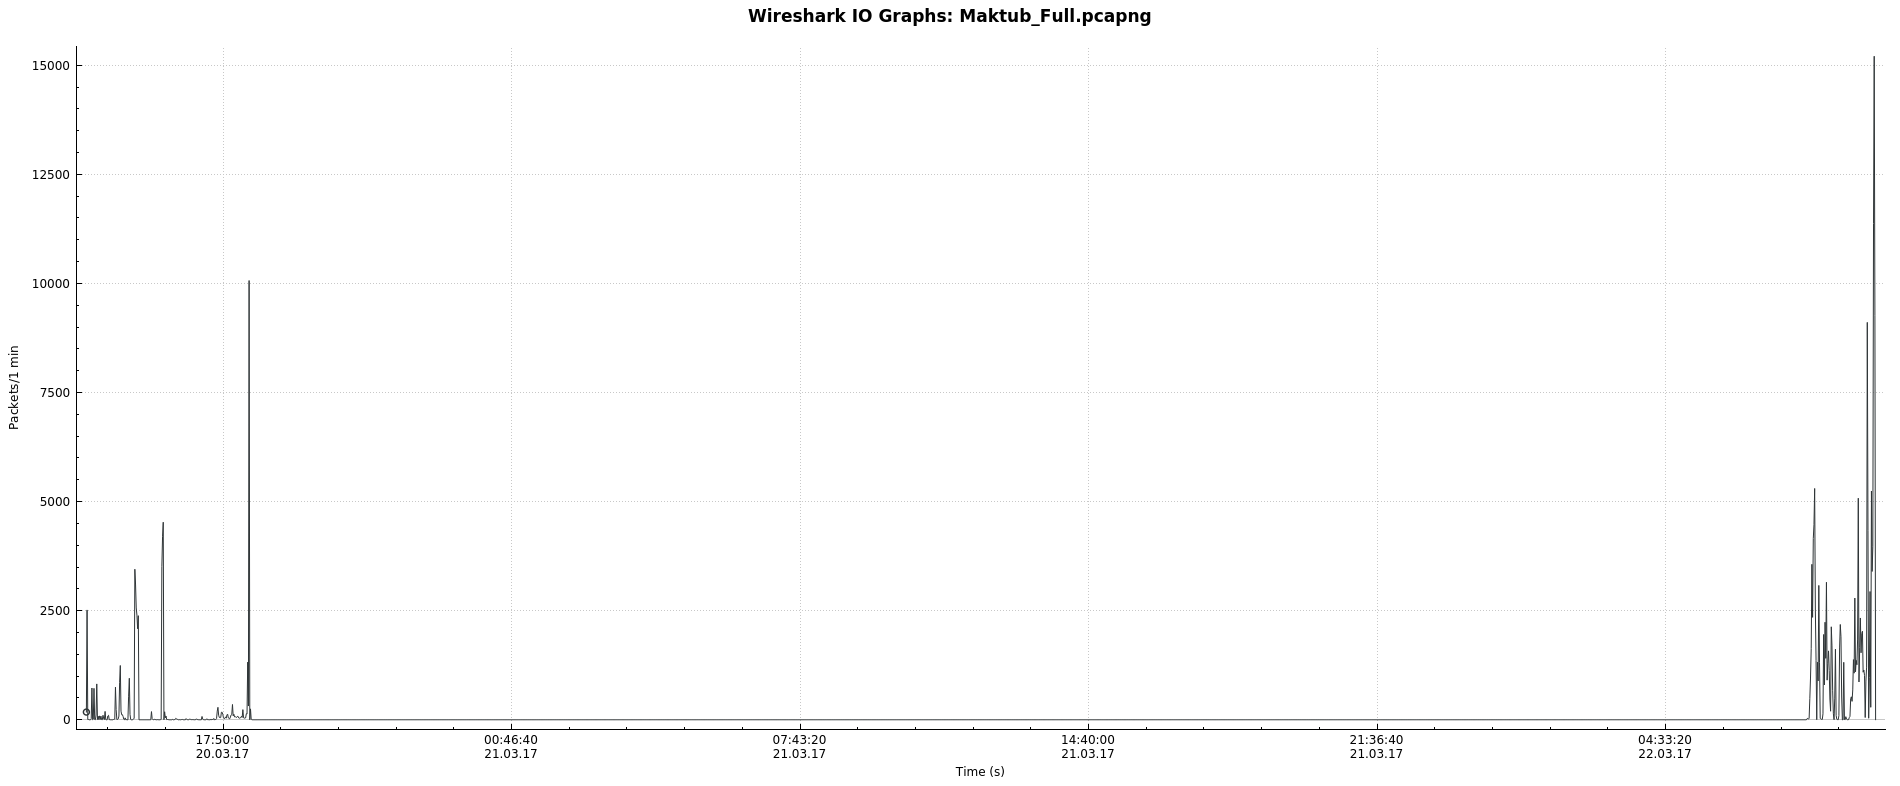
\includegraphics[scale=0.28]{Maktub_Full.png}
    \caption{Pcap Lifetime graph}
\end{figure}

\begin{figure}[H]
        \centering
        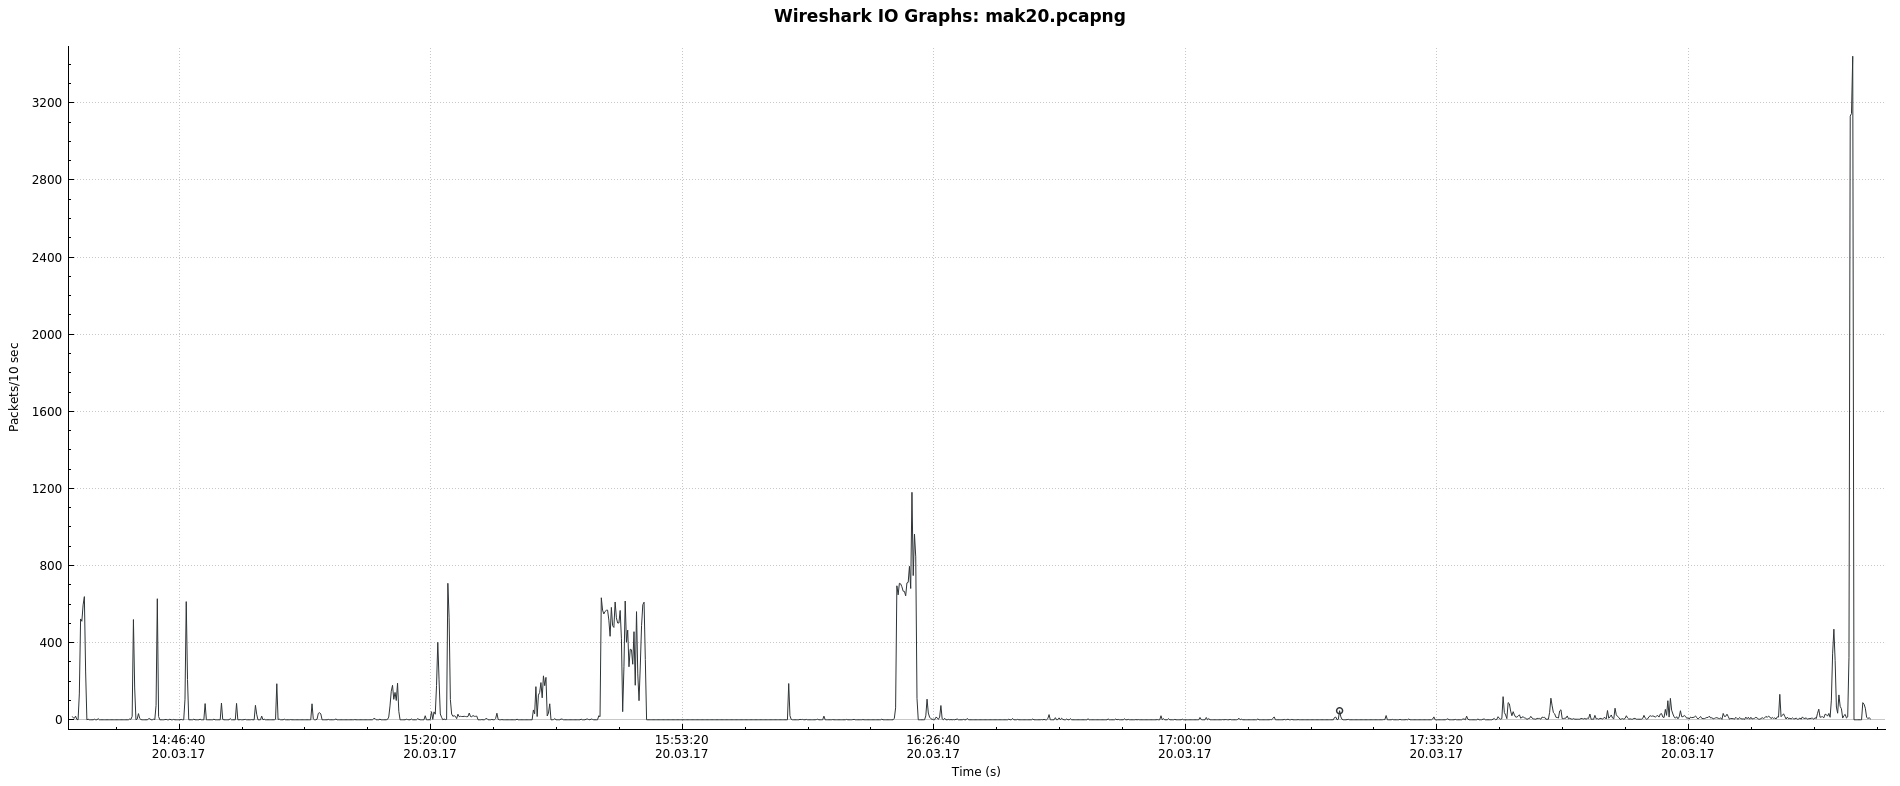
\includegraphics[scale=0.28]{mak20.png}
    \caption{IO graph for 2017-03-20} 
\end{figure}

\begin{figure}[H]
        \centering
        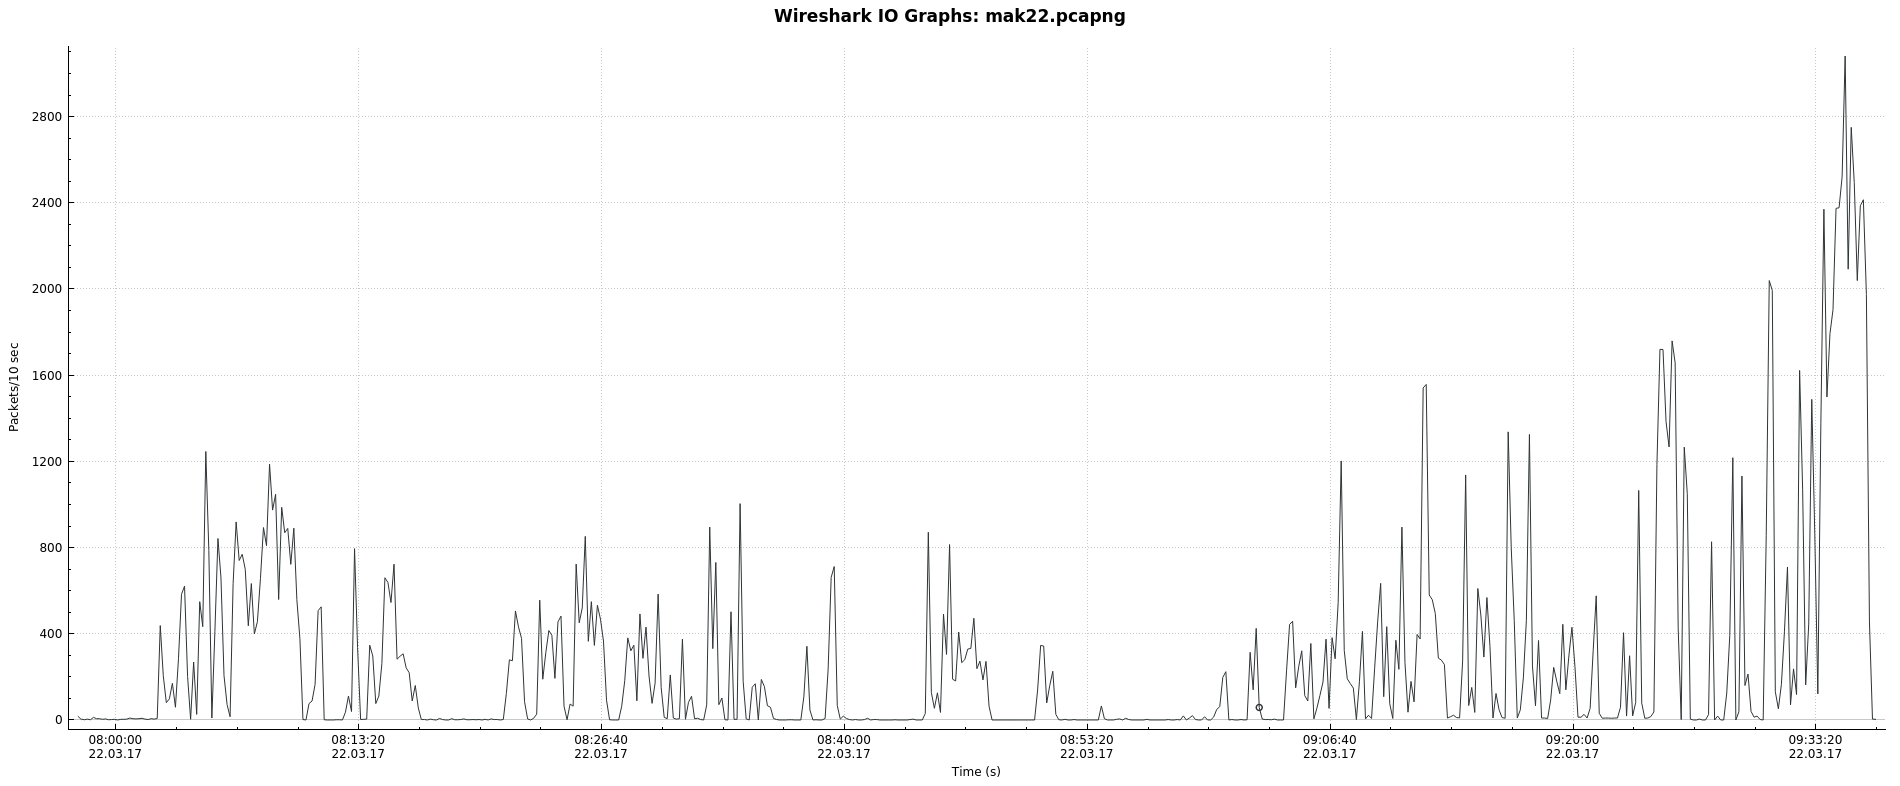
\includegraphics[scale=0.28]{mak22.png}
    \caption{IO Graph for 2017-03-22}
\end{figure}

% STANDTHIS
This analysis examines events that took place on a South African network on the 2017-03-20 and 2017-03-22. We will make the argument, based purely on captured network traffic and inferences gleaned from prior malware analysis, that a host was compromised with a ransomware variant known as Maktub. 

% DAN 
The three graphs depict packets per 10 seconds for a the compete pcap sample, followed by traffic generated on the 20th and 22nd. The traffic was divided in this way to logically separate the behavior associated with each time sequence. The story of the infected host is encapsulated on the first day, whereas the second day exhibits indirect behavior of the infected host as the machine has been taken offline.  

A point to make about attacks of this kind, is that they can easily slip between the cracks since benign traffic is by far the most dominant communication on the network. Most of the traffic generated involves the target host receiving legitimate windows updates from trusted IP addresses. 

In monitoring the DNS traffic closely we found some interesting queries for known malicious sites. We set out to uncover the initial execution point of the malicious code and how communication with the C2 (command and control server) was carried out.

Legitmate windows update from Ikai CDN 
DNS for onion domain Singapore 
DNS for cryptostorm to establish VPN Germany
Get Windows-CryptoAPI from comodoca 
China DNS req  for 1.83.255.178 

Cryptostorm VPN connect over TLS 
192.36.27.5 -> Amsterdam IP for onion (Entry node)
103.198.0.2     45jngpxc4cgsxqxc.onion.link -> Singapore

%------------------------------------------------

\section*{Traffic for initial compromise on the 20th}

% DAN
On the 2017-03-20 our host (10.0.0.5) seems to be engaged in routine Windows updates from IPs associated with Microsoft and Akamai (A legitimate CDN, content distribution network). The first signs of anomalous activity commence from what appears to be a span mail. A mail with an attachment, potentially a Microsoft Word document, is fetched after a "503 Backend fetch failed" response. The following request is made to a destination IP associated with an onion domain (Host: 45jngpxc4cgsxqxc.onion.link). The .onion domain refers to TOR hidden services which require the TOR browser to interpret the protocol and connect to the site. TOR is a privacy oriented protocol which aims to obscure the origin of the sender, by encapsulating a packet in three layers of encryption before routing the packet through three intermediaries nodes on the way to the server. The protocol serves a valuable role to actors of differing motivation. The protocol is not only used by activists and those circumventing censorship but also those who exploit it for profit. The ".link" allows for for convenience at the expense of privacy, as your service provider can see your what content you are requesting \cite{onionlink}. The host also visited  torstorm.org domain, which offers a similar service. This allowed the target system to visit a TOR hidden services hosted by our attackers. The onion link confirms our suspicions as it is associated with a malware analysis of a malicious windows executable inserted inside a benign looking update policy word document \cite{hybrid}. Please refer to appendix A for the TCP conversation of the payload delivery.

Following execution of the payload we can infer that the DNS queries were made in order to resolve another .onion domain.

\begin{lstlisting}[language=html]
("45jngpxc4cgsxqxc.torstorm.org", A(94.242.58.199))
\end{lstlisting}

Next we see a query for the domain cyrptostorm.is. Cryptostorm is a German based VPN service that markets itself as for the "truly paranoid" \cite{cryptostorm}. Cryptostorm uses openVPN to establish a secure VPN connection. The target host uses TLS to tunnel the openVPN connection to avoid blocking of the protocol. This is a feature provided by Cryptostorm which encrypts the TCP handshake to obscure the openVPN traffic \cite{tls}. 

\begin{lstlisting}
("186.240.165.46.in-addr.arpa", PTR("cryptostorm.is"))
\end{lstlisting}

The openVPN connection provides a secure communication channel for remote interaction with the host. This traffic is encrypted but DNS queries leak from the compromised host giving away precious information about the malware's behavior. We assume that this is an oversight made by the malware developers, as DNS resolution should happen over an encrypted channel.  DNS is a protocol that provides valuable insights to ISPs and intelligence agencies conducting surveillance. DNSsec provides tries to find a solution to this problem, by encrypting DNS \cite{dnssec}. 

The DNS leaks provide insights into the TOR hidden services that are being accessed via the Cryptostorm VPN. The domains queried are all associated with TOR hidden service payment portals used by attackers to receive Cryptocurrency payments \cite{hybrid}. Once again we see the use of services that allow insecure access to TOR by regular web browses. 

\begin{lstlisting}
("45jngpxc4cgsxqxc.torstorm.org", A(94.242.58.199)) 
("45jngpxc4cgsxqxc.tor2web.org", A(192.36.27.5))
\end{lstlisting}

The following illustrates what is likely to be the user checking the payment portal.
\begin{lstlisting}
00:16:6f:98:80:74 -> c8:51:95:2c:35:73, [tcp] 10.0.0.5:49219         -> 192.36.27.5:80         [http] Request { method: "GET", uri: "/", version: "1.1", host: Some("45jngpxc4cgsxqxc.tor2web.org"), agent: Some("Mo
zilla/4.0 (compatible; MSIE 8.0; Windows NT 6.1; Trident/4.0; SLCC2; .NET CLR 2.0.50727; .NET CLR 3.5.30729; .NET CLR 3.0.30729; Media Center PC 6.0; InfoPath.2)"), referer: None, auth: None, cookies: None }
\end{lstlisting}

The target host ceases to exist on the networking failing to respond to even ARP broadcasts from this point fordard. 

%Tor2web listing

Windows NT 6.1

Malicious IPs 
103.198.0.2:80
192.36.27.5:443
192.36.27.5:80
192.64.119.254:80


%------------------------------------------------

\section*{Traffic captured on the 22nd}

The target host appears to have been taken offline by the user. Traffic generated on the 22nd is primarily benign windows updates and legitimate web traffic from other hosts on the network. Although no malicious connections were established, there were abnormal ARP probes.

The default gateway 10.0.0.2 broadcasted asking for compromised host. The broadcast was made 485 times. This could possibly indicate the command and control server attempting to reestablish communication with the target, as the default gateway attempted to ARB probe for the host. This assumes that the network has no firewall in place, or one that is misconfigured. Since packets entering the network should be blocked unless they are solicited from inside the network, as part of an on going connection. Thus the best explanation for the anomalous ARP probes are that the C2 server is checking whether his compromised hosts are still online.

%------------------------------------------------

\section*{Conclusion}

%----------------------------------------------------------------------------------------
%	BIBLIOGRAPHY
%----------------------------------------------------------------------------------------

\clearpage
%\bibliographystyle{unsrt}
\bibliographystyle{plainnat}
%plainnat, unsrtnat and abbrevnat)
\bibliography{paper.bib}

\section*{Appendix A}
\lstinputlisting[language=html]{mailreq.txt}

%----------------------------------------------------------------------------------------

\end{document}
